% --- LaTeX Presentation Template - S. Venkatraman ---

% --- Set document class ---

% Remove "handout" when presenting to include pauses
\documentclass[dvipsnames, handout]{beamer}
\usetheme{default}

% Make content that is hidden by pauses "transparent"
\setbeamercovered{transparent}

% --- Slide layout settings ---

% Set line spacing
\renewcommand{\baselinestretch}{1.15}

% Set left and right text margins
\setbeamersize{text margin left=12mm, text margin right=12mm}

% Add slide numbers in bottom right corner
\setbeamertemplate{footline}[frame number]

% Remove navigation symbols
\setbeamertemplate{navigation symbols}{}

% Allow local line spacing changes
\usepackage{setspace}

% Change itemized list bullets to circles
\setbeamertemplate{itemize item}{$\bullet$}
\setbeamertemplate{itemize subitem}{$\circ$}

% --- Color and font settings ---

\usepackage{xcolor}

% Slide title background color
\definecolor{background}{HTML}{ede6d8}

% Slide title text color
\definecolor{titleText}{HTML}{9e1c33}
\definecolor{white}{HTML}{ffffff}

% Other possible color schemes

% - Light green/dark green -
%\definecolor{background}{HTML}{e4ede4}
%\definecolor{titleText}{HTML}{2e592f}

% - Light blue/dark blue -
%\definecolor{background}{HTML}{d5d9e8}
%\definecolor{titleText}{HTML}{2d375e}

% - Beige/dark blue -
%\definecolor{background}{HTML}{e8e2d5}
%\definecolor{titleText}{HTML}{2d3375}

% Set colors
\setbeamercolor{frametitle}{bg=titleText, fg=white}
\setbeamercolor{subtitle}{fg=titleText}

% Set font sizes for frame title and subtitle
\setbeamerfont{frametitle}{size=\fontsize{15}{16}}
\setbeamerfont{framesubtitle}{size=\small}

% --- Math/Statistics commands ---

% Add a reference number to a single line of a multi-line equation
% Usage: "\numberthis\label{labelNameHere}" in an align or gather environment
\newcommand\numberthis{\addtocounter{equation}{1}\tag{\theequation}}

% Shortcut for bold text in math mode, e.g. $\b{X}$
\let\b\mathbf

% Shortcut for bold Greek letters, e.g. $\bg{\beta}$
\let\bg\boldsymbol

% Shortcut for calligraphic script, e.g. %\mc{M}$
\let\mc\mathcal

% \mathscr{(letter here)} is sometimes used to denote vector spaces
\usepackage[mathscr]{euscript}

% Convergence: right arrow with optional text on top
% E.g. $\converge[p]$ for converges in probability
\newcommand{\converge}[1][]{\xrightarrow{#1}}

% Weak convergence: harpoon symbol with optional text on top
% E.g. $\wconverge[n\to\infty]$
\newcommand{\wconverge}[1][]{\stackrel{#1}{\rightharpoonup}}

% Equality: equals sign with optional text on top
% E.g. $X \equals[d] Y$ for equality in distribution
\newcommand{\equals}[1][]{\stackrel{\smash{#1}}{=}}

% Normal distribution: arguments are the mean and variance
% E.g. $\normal{\mu}{\sigma}$
\newcommand{\normal}[2]{\mathcal{N}\left(#1,#2\right)}

% Uniform distribution: arguments are the left and right endpoints
% E.g. $\unif{0}{1}$
\newcommand{\unif}[2]{\text{Uniform}(#1,#2)}

% Independent and identically distributed random variables
% E.g. $ X_1,...,X_n \iid \normal{0}{1}$
\newcommand{\iid}{\stackrel{\smash{\text{iid}}}{\sim}}

% Sequences (this shortcut is mostly to reduce finger strain for small hands)
% E.g. to write $\{A_n\}_{n\geq 1}$, do $\bk{A_n}{n\geq 1}$
\newcommand{\bk}[2]{\{#1\}_{#2}}

% Math mode symbols for common sets and spaces. Example usage: $\R$
\newcommand{\R}{\mathbb{R}}	% Real numbers
\newcommand{\C}{\mathbb{C}}	% Complex numbers
\newcommand{\Q}{\mathbb{Q}}	% Rational numbers
\newcommand{\Z}{\mathbb{Z}}	% Integers
\newcommand{\N}{\mathbb{N}}	% Natural numbers
\newcommand{\F}{\mathcal{F}}	% Calligraphic F for a sigma algebra
\newcommand{\El}{\mathcal{L}}	% Calligraphic L, e.g. for L^p spaces

% Math mode symbols for probability
\newcommand{\pr}{\mathbb{P}}	% Probability measure
\newcommand{\E}{\mathbb{E}}	% Expectation, e.g. $\E(X)$
\newcommand{\var}{\text{Var}}	% Variance, e.g. $\var(X)$
\newcommand{\cov}{\text{Cov}}	% Covariance, e.g. $\cov(X,Y)$
\newcommand{\corr}{\text{Corr}}	% Correlation, e.g. $\corr(X,Y)$
\newcommand{\B}{\mathcal{B}}	% Borel sigma-algebra

% Other miscellaneous symbols
\newcommand{\tth}{\text{th}}	% Non-italicized 'th', e.g. $n^\tth$
\newcommand{\Oh}{\mathcal{O}}	% Big-O notation, e.g. $\O(n)$
\newcommand{\1}{\mathds{1}}	% Indicator function, e.g. $\1_A$

% Additional commands for math mode
\DeclareMathOperator*{\argmax}{argmax}	% Argmax, e.g. $\argmax_{x\in[0,1]} f(x)$
\DeclareMathOperator*{\argmin}{argmin}	% Argmin, e.g. $\argmin_{x\in[0,1]} f(x)$
\DeclareMathOperator*{\spann}{Span}	% Span, e.g. $\spann\{X_1,...,X_n\}$
\DeclareMathOperator*{\bias}{Bias}	% Bias, e.g. $\bias(\hat\theta)$
\DeclareMathOperator*{\ran}{ran}		% Range of an operator, e.g. $\ran(T) 
\DeclareMathOperator*{\dv}{d\!}		% Non-italicized 'with respect to', e.g. $\int f(x) \dv x$
\DeclareMathOperator*{\diag}{diag}	% Diagonal of a matrix, e.g. $\diag(M)$
\DeclareMathOperator*{\trace}{trace}	% Trace of a matrix, e.g. $\trace(M)$
\DeclareMathOperator*{\supp}{supp}	% Support of a function, e.g., $\supp(f)$

% --- Presentation begins here ---

\begin{document}

% --- Title slide ---

\title{\color{titleText}Mobile Machine Learning}
\author{Ruben Teimas\vspace{-.3cm}}
\institute{Universidade de Évora, Ubiquitous Computing}

\begin{frame}
\titlepage
\vspace{-1.2cm}
\begin{center}

\includegraphics[width=2.3cm]{presentation/uevora_logo.png}\bigskip
\date{\today}
\end{center}
\end{frame}


% --- Main content ---

% Example slide: use \pause to sequentially unveil content

%%%%% Mobile %%%%%%%%%%%%%%%%%%%%%%

\begin{frame}{What are mobile devices?}
Even though there is no exact definition, they (usually) share some characteristics: 
\pause
\begin{itemize}
\item Touchscreen interfaces with color display;
\item Rechargeable batteries;
\item Can connect over wireless networks.
\end{itemize}
\end{frame}

\begin{frame}{Example of mobile devices}
\begin{center}
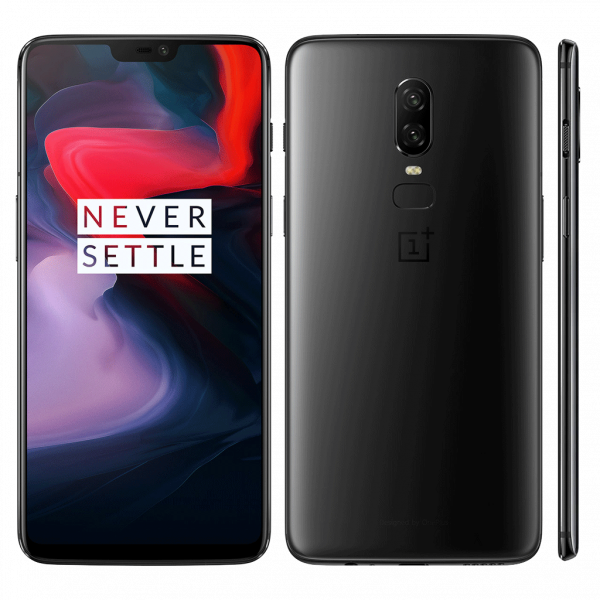
\includegraphics[scale=0.2]{presentation/one_plus.png}
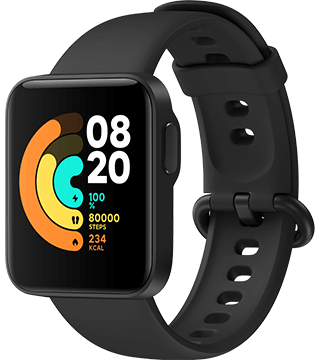
\includegraphics[scale=0.2]{presentation/watch.png}  
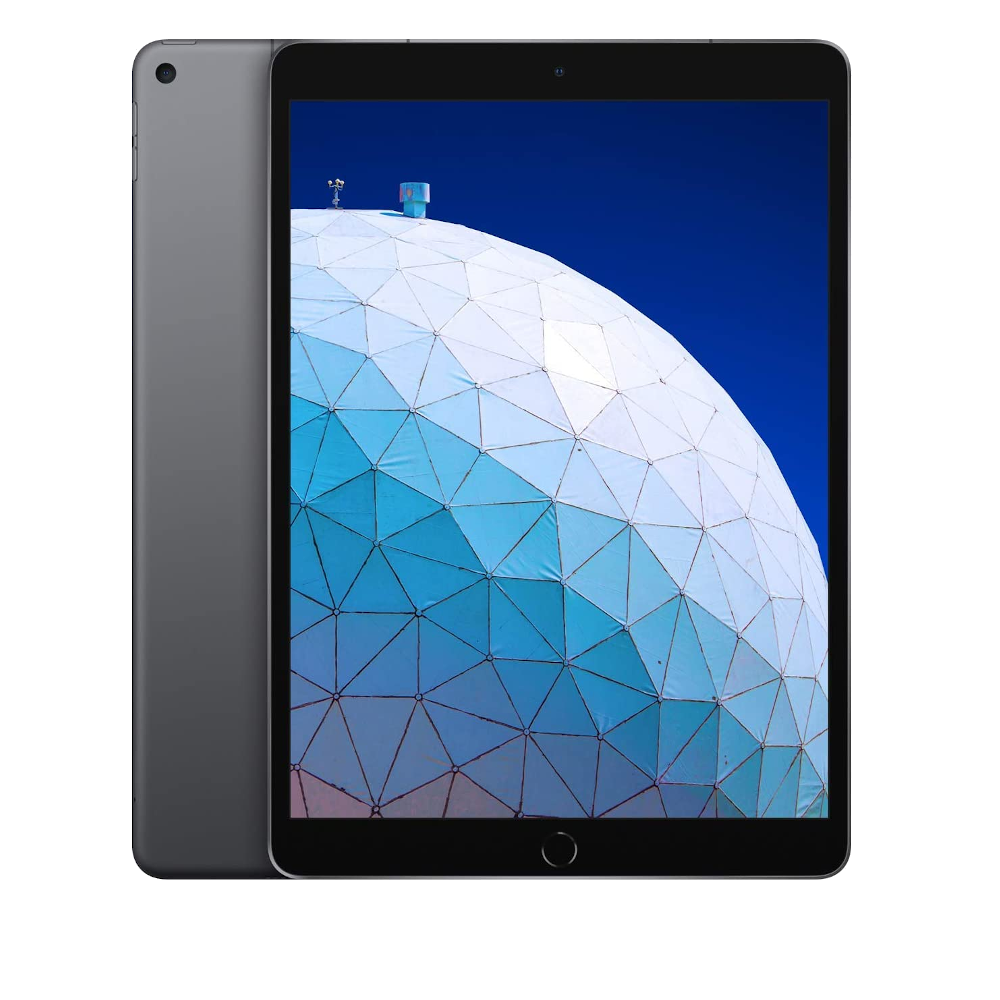
\includegraphics[scale=0.4]{presentation/ipad.png}  
\end{center}
\pause
The perception of mobile devices are has changed over the years and some people do not consider the \emph{Tablet} to be a mobile device anymore.
\end{frame}

\begin{frame}{The rise of mobile devices}
Impactful events for the rise of mobile devices:
\pause
\begin{itemize}
    \item Presentation of the \emph{IPhone} (2007);
    \item \emph{Android} \emph{os} launching (2008).
\end{itemize}
\pause
These events changed the perception of what a phone should be, making it closer to equipment of the time, like the \emph{IPod} and \emph{PDA}s, but still with everything a traditional phone had to offer.
\end{frame}

\begin{frame}{The rise of mobile devices}
\begin{center}
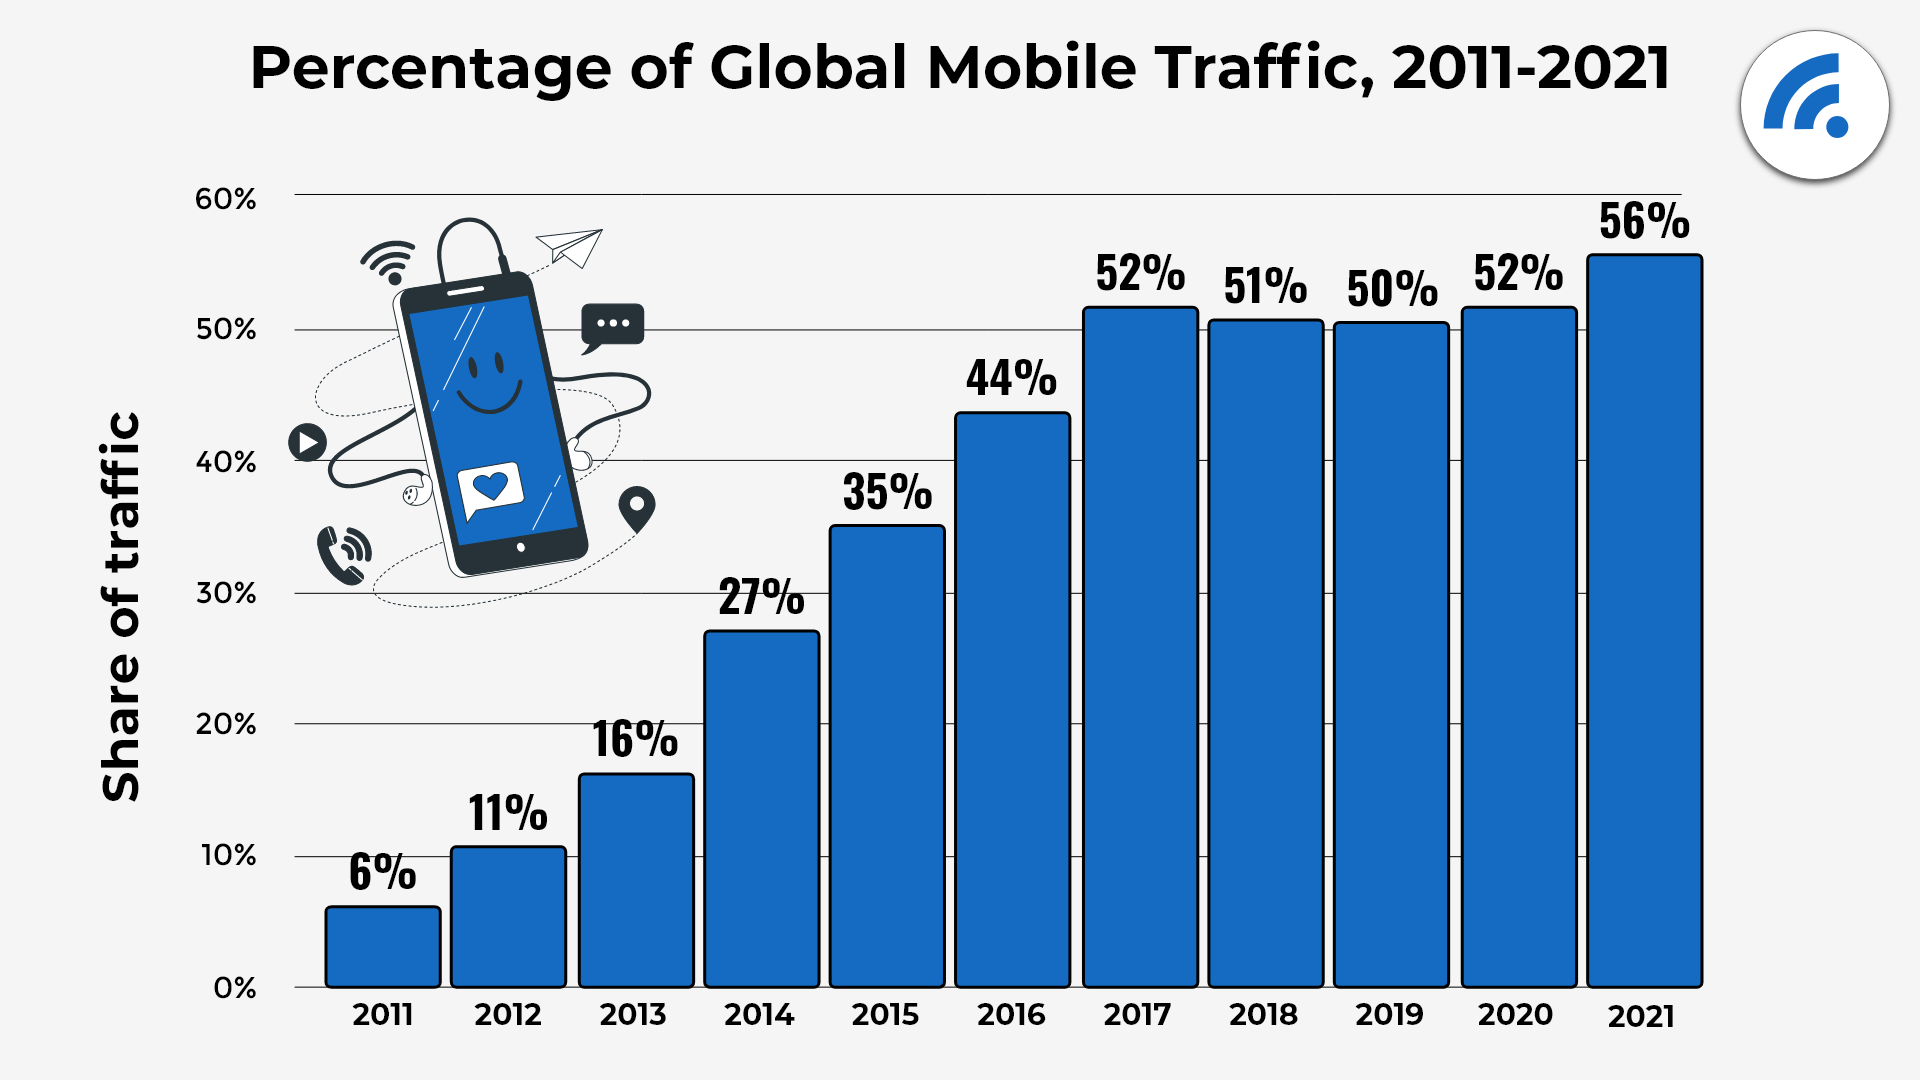
\includegraphics[scale=0.15]{presentation/mobile_traffic.png}
\end{center}
\pause
\end{frame}

%%%%% Machine Learning %%%%%%%%%%%%%%%%%%%%%%
\begin{frame}{\emph{Artificial Intelligence and Machine Learning}}
The terms \emph{AI} and \emph{ML} almost always appear together, which misleads some people to believe they are the same thing.
\begin{center}
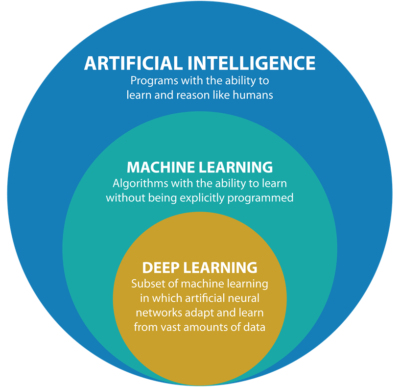
\includegraphics[scale=0.5]{presentation/ml_def.png}
\end{center}
\pause
\end{frame}

\begin{frame}{The beginning}
Even thought \emph{Machine Learning} has only achieved commercial success in 2010's it has been around since the 50's.
\pause
\begin{center}
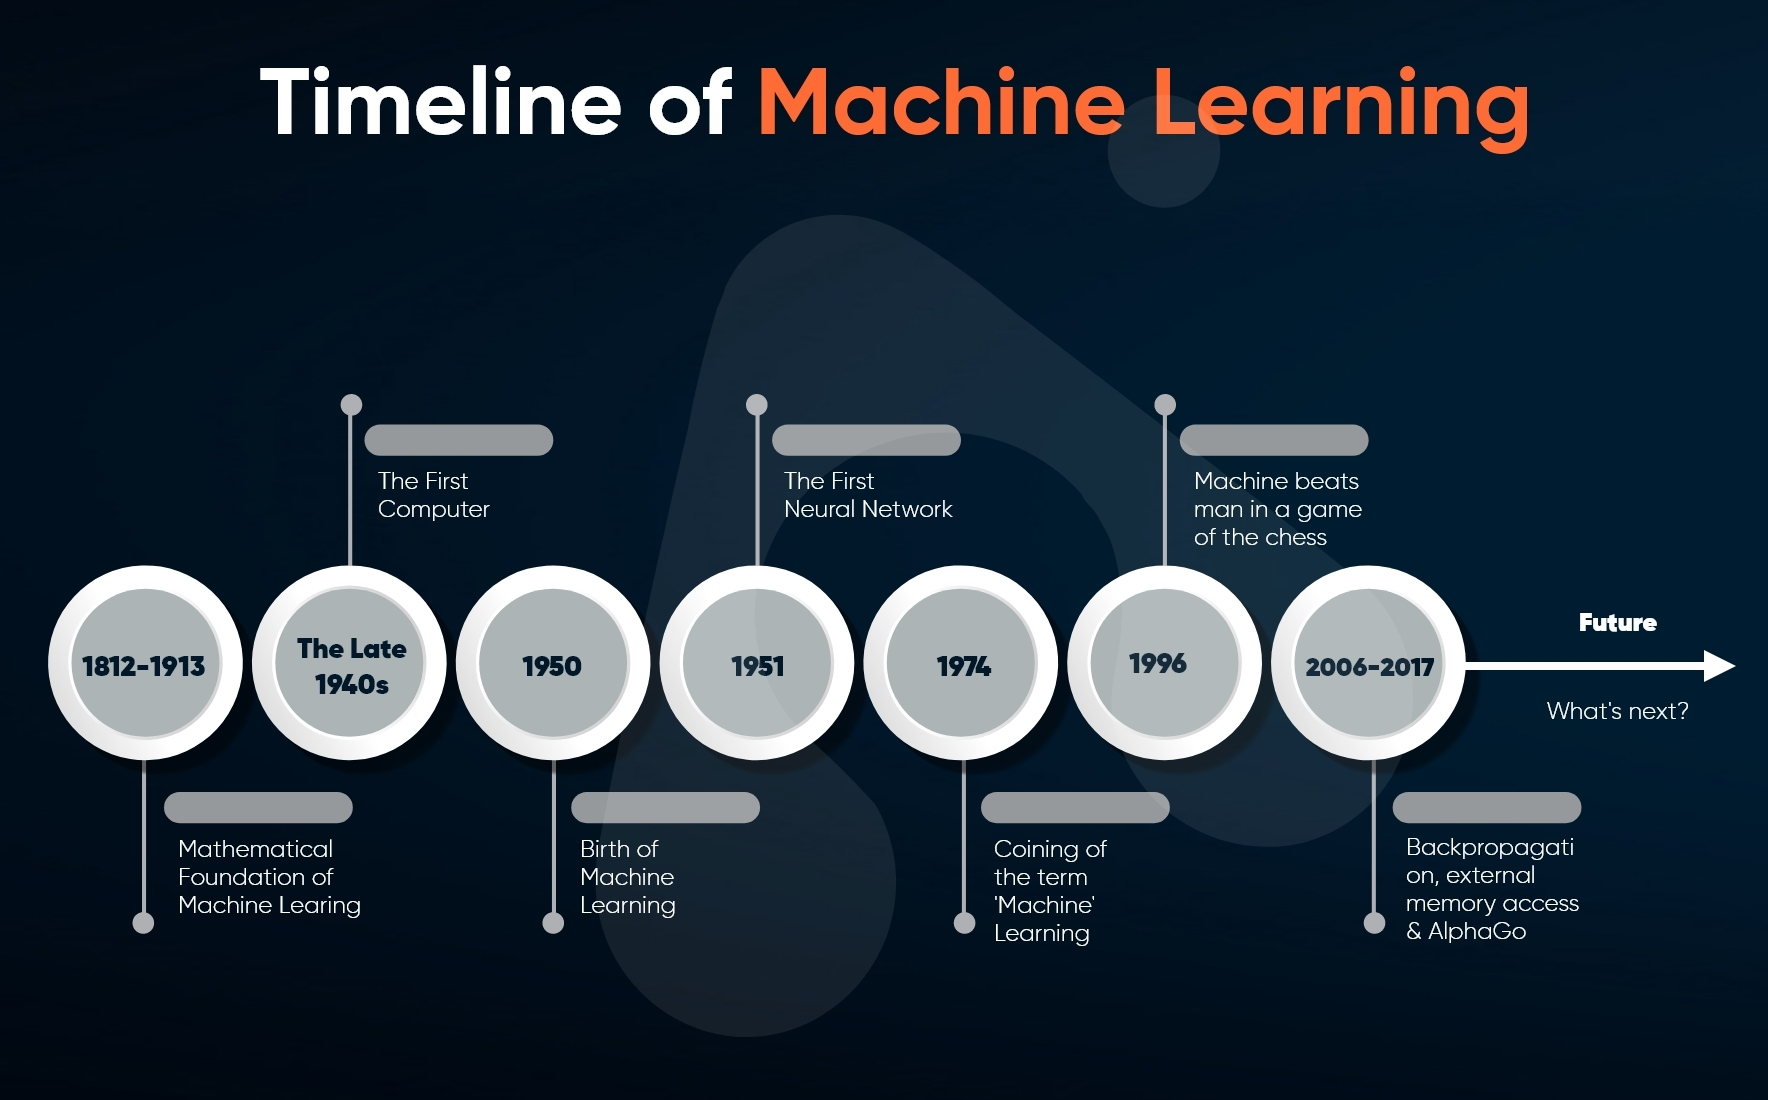
\includegraphics[scale=0.15]{presentation/timeline.jpg}
\end{center}
\pause
\end{frame}

\begin{frame}{\emph{Where we're at}}
Fortunately \emph{ML} has evolved immensely over the years and has given us:
\pause
\begin{center}
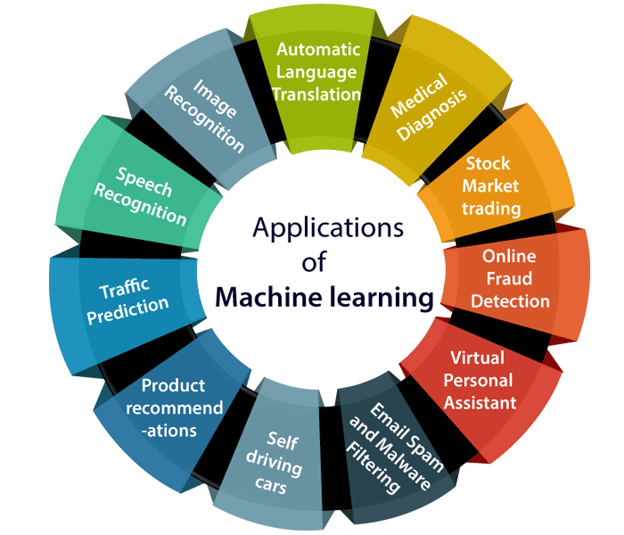
\includegraphics[scale=0.2]{presentation/ml_now.png}
\end{center}
\pause
\end{frame}


\begin{frame}{What made it possible?}
Large volumes of data and hardware's improvement gave \emph{ML} the possibility to shine.\\
\pause
\\
Cloud computing has also played a big part in \emph{machine learning} development, making it easier to train models on large clusters (with fast \emph{CPU}s and lots of \emph{GPU}s).
\pause
\end{frame}

\begin{frame}{Technologies}
Some of the technologies that have made \emph{ML} easier to train and develop:
\pause
\begin{center}

\includegraphics[scale=0.2]{presentation/cuda.jpg}

\includegraphics[scale=0.12]{presentation/tf.png}  

\includegraphics[scale=0.1]{presentation/scikit.png}  
\end{center}
\pause
\end{frame}
%%%%%%%%%%%%%%%%%%%%%%%% Both %%%%%%%%%%%%%%%%%%%%
\begin{frame}{Data Collection}
Data is \emph{Machine Learning}'s fuel.
\pause
\begin{center}
\pause
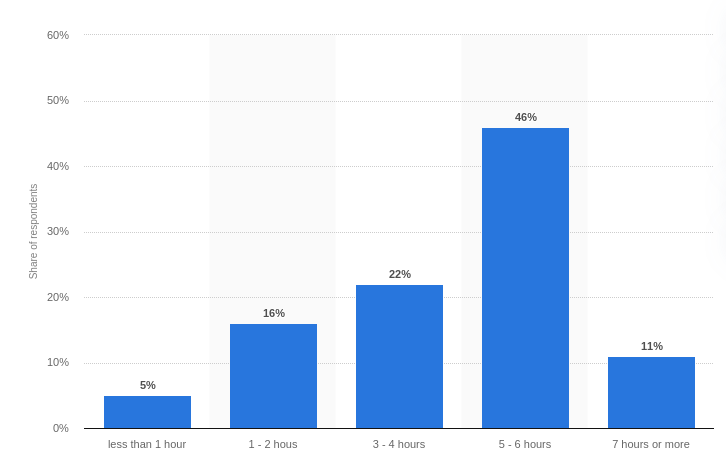
\includegraphics[scale=0.3]{presentation/Screenshot from 2021-05-25 13-06-19.png}
\end{center}
\pause
A person living in the \emph{USA} spends, on average, 3,5 hours on their phone, thus making it a good source of data by keeping track of user's behaviour. 
\end{frame}

\begin{frame}{\emph{ML} on Mobile}
Thanks to \emph{Google}, \emph{Machine Learning} development for \emph{Mobile} is easier than ever.
\pause
Some of the technologies that can be used to integrate \emph{ML} into \emph{mobile apps} are:
\begin{itemize}
    \item \emph{ML Kit}.
    \item \emph{TensorFlow Lite}.
\end{itemize}
\pause
\end{frame}

\begin{frame}{\emph{ML} on Mobile}
If \emph{Cloud Computing} has been extremely important for \emph{Machine Learning}, one of the newest trends in \emph{On-Device} training (which both these tools allow).\\
\pause
Today's mobile devices are very powerful and have the capability to train models.
\end{frame}

\begin{frame}{Advantages of \emph{On-Device} training}
\begin{itemize}
    \item Increased privacy;
    \item No internet connection is required;
    \item Decreased latency, since there is no communication with the server. 
\end{itemize}
\end{frame}

\begin{frame}{\emph{ML} on Mobile}
\pause
\begin{center}
\pause
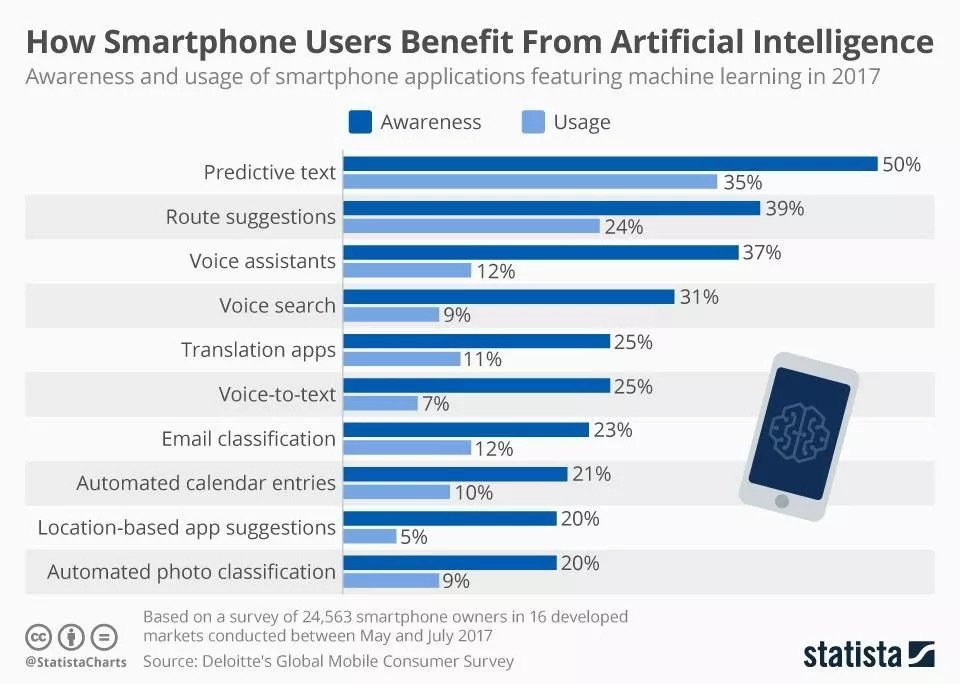
\includegraphics[scale=0.3]{mobile_apps.jpg}
\end{center}
\pause
\end{frame}

\begin{frame}{Brave new world}
\pause
\emph{Internet of Things} (\emph{IoT}) connects multiple devices (with embedd sensors and software) over the network. 
\begin{center}
\pause
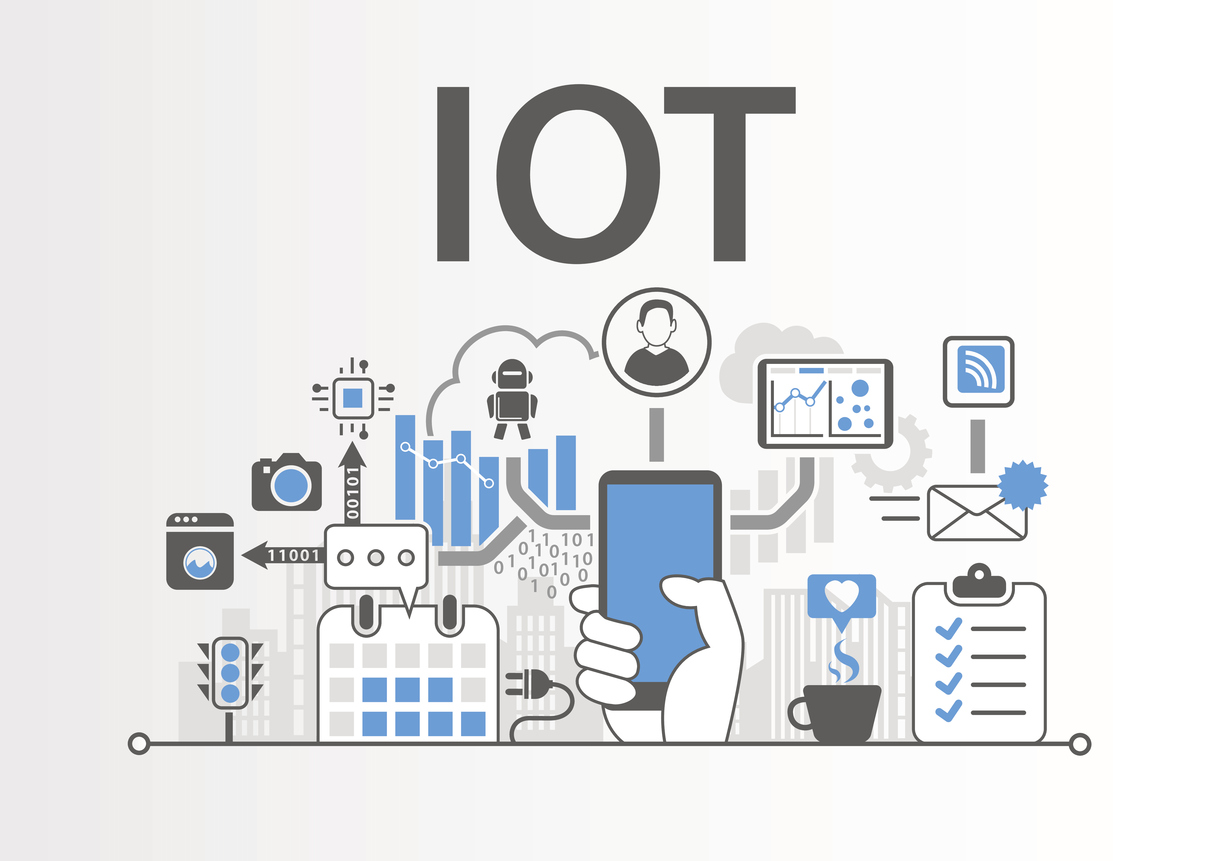
\includegraphics[scale=0.6]{presentation/iot.jpg}
\end{center}
\pause
Usually these devices can be controlled via \emph{smartphone}.
\end{frame}

\begin{frame}{Brave new world}
\emph{ML} is now being applied to \emph{IoT} devices, for example:
\begin{itemize}
    \item \emph{Google Assistant}
    \item \emph{Nest Thermostat}
\end{itemize}
\end{frame}

\begin{frame}{Future perceptive}
The way we interact with technology, and the world, has been changing and will, most likely, keep changing towards a more fluid experience. 

This is possible due to \emph{mobile devices}, making our computer smaller and smaller, and to \emph{ml} which creates more intelligent and "\emph{humanized}" systems.
\end{frame}

% --- Thank you slide ---

\begin{frame}
\begin{center}
{\large\color{titleText} Thank you for listening!}
\vspace{1cm}

Ruben Teimas\\[1em]
m47753@alunos.uevora.pt \\
https://github.com/TeimasTeimoso \\
https://www.linkedin.com/in/ruben-teimas/
\end{center}
\end{frame}

% --- Presentation ends here ---

\end{document}
